\documentclass[a4paper,11pt,twoside]{report}
%%\usepackage{program}
\usepackage{amsmath}
\usepackage{ascmac}
\usepackage[dvipdfmx]{graphicx}  % for EPS and PDF 
\usepackage{url}
\usepackage{fancyvrb}
\usepackage{makeidx}
\usepackage{here}
\usepackage[dvipdfmx]{color}
\usepackage{ulem}
%\usepackage[sectionbib]{chapterbib}

\usepackage{vruler}  %% if vertical ruler (line number) is needed

%\usepackage[dvipdfm,bookmarkstype=toc,colorlinks=true,urlcolor=black,%
%    linkcolor=black,citecolor=black,linktocpage=true,bookmarks=false]{hyperref}
%\usepackage[dvipdfm,bookmarkstype=toc,colorlinks=true,urlcolor=black,%
%    linkcolor=black,citecolor=black,bookmarks=false]{hyperref}
\usepackage[dvipdfm,bookmarkstype=toc,urlcolor=black,%
    linkcolor=black,citecolor=black,bookmarks=false]{hyperref}

\setcounter{secnumdepth}{4}
\setcounter{totalnumber}{6}
\usepackage{fancyhdr}


\hoffset=0cm
\oddsidemargin=0cm
\evensidemargin=0cm
\textwidth=16cm
%\topmargin=-1.5cm
\topmargin=-1cm
\voffset=0cm
\textheight=24cm

\long\def\comment#1{}
\def\progenv{\baselineskip=10pt\tt\progspecial{`}\parindent=0.3cm}
\def\shellenv{\baselineskip=10pt\tt\progspecial{`}\parindent=0.3cm\nolineno}

%%\renewcommand{\topfraction}{0.85}
%%\renewcommand{\textfraction}{0.1}
%%\renewcommand{\floatpagefraction}{0.75}

\renewcommand{\topfraction}{.99}
\renewcommand{\bottomfraction}{.99}

\def\openb{{\it [}}
\def\closeb{{\it ]}}
%\def\openp{{\tt (}}
%\def\closep{{\tt )}}

\def\DAG{$^\dagger$}
\def\DDAG{$^\ddagger$}

\def\XMP{XcalableMP}
\def\OMP{OpenMP}
\def\HPF{HPF}
\def\CAF{Co-array Fortran}
\def\MPI{MPI}
\def\Fort{Fortran}
\def\C{C}
\def\XMPF{XcalableMP Fortran}
\def\XMPC{XcalableMP C}

\def\Directive#1{{\tt #1}\index{#1@{\tt #1}}\index{Directive!#1@{\tt #1}}}

%\def\Syntax#1{\index{{\tt #1}}\index{Syntax!{\tt #1}}}
\def\Syntax#1{\index{Syntax!#1@{\tt #1}}}

\def\Term#1{{#1}\index{#1}}

%\def\Example#1{\index{#1}\index{Example!{\tt #1}}}
\def\Example#1{\index{Example!#1@{\tt #1}}}

\def\Intrinsic#1{\index{#1@{\tt #1}}\index{Intrinsic and Library Procedures!#1@{\tt #1}}}

\def\NULL{{\tt NULL}}

\def\PROG#1{{\tt #1}\index{\tt #1}\index{Command!#1}}
\def\FUNC#1{{\tt #1()}\index{\tt #1}\index{Example Function!#1}}
\def\LPROG#1{{\tt #1}\index{\tt #1}\index{Linux Command!#1}}
\def\LFUNC#1{{\tt #1()}\index{\tt #1}\index{Linux Function!#1}}
\def\MFUNC#1{{\tt #1()}\index{\tt #1}\index{Myrinet/MX Function!#1}}
\def\SFUNC#1{{\tt #1()}\index{\tt #1}\index{Sample Code!#1}}
\def\STRUCT#1{{\tt #1}\index{\tt #1}\index{Struct!#1}}
\def\VAR#1{{\tt #1}\index{\tt #1}\index{Variable!#1}}
\def\ARG#1{{\tt #1}\index{\tt #1}\index{Variable!#1}}
\def\MACRO#1{{\tt #1}\index{\tt #1}\index{Macro!#1}}
\def\ERRNO#1{{\tt #1}\index{\tt #1}\index{ERRNO!#1}}
\def\SIGNAL#1{{\tt #1}\index{\tt #1}\index{Signal!#1}}
\def\FILE#1{{\tt #1}\index{\tt #1}\index{File!#1}}
\def\ENV#1{{\tt #1}\index{\tt #1}\index{Environment Variable!#1}}
\def\INDEX#1{#1\index{#1}}
\def\OPTION#1{{\tt #1}\index{Command Option!#1}}
\def\TERM#1{\underline{#1}\index{#1}}
\def\CTRL#1{{\tt $^\wedge$#1}}

\def\phrule{\vspace{0.2cm}\hrule\vspace{0.05cm}\hrule}
\def\qhrule{\vspace{0.2cm}\hrule}

\def\dhrule{\hrule\vspace{0.05cm}\hrule}

\def\bsquare{\rule[-2pt]{5pt}{10pt}}

\newcommand\gio{{\tt global\_io }}
\newcommand\mio{{\tt master\_io }}

\newcommand{\mytextcolor}[2]{\textcolor{#1}{#2}}
%\newcommand{\mytextcolor}[2]{{#2}}
\newcommand{\mycolor}[1]{\color{#1}}

\newenvironment{point}[1]{\vspace*{0.3cm}\begin{itembox}{#1}}{\end{itembox}\vspace*{0.3cm}}

\newenvironment{note}[1]{\vspace*{0.3cm}\begin{itembox}{Note on #1}}{\end{itembox}\vspace*{0.3cm}}

\newenvironment{issue}[1]{\vspace*{0.3cm}\begin{itembox}{Issues on #1}}{\end{itembox}\vspace*{0.3cm}}

\newenvironment{errors}{\vspace*{0.3cm}\begin{tabular}{ll}\multicolumn{2}{l}{\bf Return Values}\\}{\end{tabular}\vspace*{0.3cm}}

\newenvironment{mytable}[3]{\begin{table}[ht]\caption{#1}\label{#2}\vspace*{-0.3cm}\begin{center}\begin{tabular}{#3}}{\end{tabular}\end{center}\end{table}}

\newenvironment{myfigure}{\begin{figure}[ht]\begin{center}}{\end{center}\end{figure}}

\DefineVerbatimEnvironment{Fexample}{Verbatim}{numbers=left,numbersep=3pt,stepnumber=5,frame=single,label=\Fort}

\DefineVerbatimEnvironment{FexampleR}{Verbatim}{numbers=right,numbersep=3pt,stepnumber=5,frame=single,label=\Fort}

\DefineVerbatimEnvironment{Cexample}{Verbatim}{numbers=left,numbersep=3pt,stepnumber=5,frame=single,label=\C}

\DefineVerbatimEnvironment{CexampleR}{Verbatim}{numbers=right,numbersep=3pt,stepnumber=5,frame=single,label=\C}

\DefineVerbatimEnvironment{XFexample}{Verbatim}{numbers=left,numbersep=3pt,stepnumber=5,frame=single,label=\XMPF}

\DefineVerbatimEnvironment{XFexampleR}{Verbatim}{numbers=right,numbersep=3pt,stepnumber=5,frame=single,label=\XMPF}

\DefineVerbatimEnvironment{XCexample}{Verbatim}{numbers=left,numbersep=3pt,stepnumber=5,frame=single,label=\XMPC}

\DefineVerbatimEnvironment{XCexampleR}{Verbatim}{numbers=right,numbersep=3pt,stepnumber=5,frame=single,label=\XMPC}

%% End of Preemble

\title{{\Huge XcalableMP}\\
$\langle${\it ex-scalable-em-p}$\rangle$\\
Language Specification\\
%Application Program Interface\\
\vspace{2cm}
Version 2.0 DRAFT\\}
%DRAFT 0.7}
\author{
\Large XcalableMP Specification Working Group\\
}
\date{\vspace{4cm}\Large November, 2016}

\makeindex

\begin{document}
\maketitle

Copyright \copyright 2008-2016 {\XMP} Specification Working Group.
Permission to copy without fee all or part of this material is granted,
provided the {\XMP} Specification Working Group copyright notice and the
title of this document appear. Notice is given that copying is by permission
of {\XMP} Specification Working Group.

% \clearpage
% \input{history.tex}
% \cleardoublepage

\pagenumbering{roman}
\tableofcontents
\listoffigures
\listoftables
%%%%\listoftables

\chapter*{Acknowledgment}

The specification of {\XMP} is designed by the {\XMP} Specification
Working Group, which consists of the following members from academia,
research laboratories, and industries.

\begin{itemize}
\setlength{\itemsep}{-1mm}
\item Tatsuya Abe        \dotfill \ RIKEN
\item Tokuro Anzaki      \dotfill \ Hitachi
\item Taisuke Boku       \dotfill \ University of Tsukuba
\item Toshio Endo        \dotfill \ TITECH
\item Yoshinari Fukui    \dotfill \ JAMSTEC
\item Yasuharu Hayashi   \dotfill \ NEC
\item Atsushi Hori       \dotfill \ RIKEN
\item Kohichiro Hotta    \dotfill \ Fujitsu
\item Hidetoshi Iwashita \dotfill \ RIKEN
\item Susumu Komae       \dotfill \ AXE
\item Atsushi Kubota     \dotfill \ Hiroshima City University
\item Jinpil Lee         \dotfill \ University of Tsukuba
\item Toshiyuki Maeda    \dotfill \ RIKEN
\item Motohiko Matsuda   \dotfill \ RIKEN
\item Yuichi Matsuo      \dotfill \ JAXA
\item Kazuo Minami       \dotfill \ RIKEN
\item Shoji Morita       \dotfill \ AXE
\item Hitoshi Murai      \dotfill \ RIKEN
\item Kengo Nakajima     \dotfill \ University of Tokyo
\item Takashi Nakamura   \dotfill \ JAXA
\item Tomotake Nakamura  \dotfill \ RIKEN
\item Mamoru Nakano      \dotfill \ CRAY
\item Masahiro Nakao     \dotfill \ RIKEN
\item Takeshi Nanri      \dotfill \ Kyusyu University
\item Kiyoshi Negishi    \dotfill \ Hitachi
\item Satoshi Ohshima    \dotfill \ University of Tokyo
\item Yasuo Okabe        \dotfill \ Kyoto University
\item Hitoshi Sakagami   \dotfill \ NIFS
\item Tomoko Sakari      \dotfill \ Fujitsu
\item Shoich Sakon       \dotfill \ NEC
\item Mitsuhisa Sato     \dotfill \ University of Tsukuba
\item Taizo Shimizu      \dotfill \ PC Cluster Consortium
\item Takenori Shimosaka \dotfill \ RIKEN
\item Yoshihisa Shizawa  \dotfill \ RIST
\item Shozo Takeoka      \dotfill \ AXE
\item Hitoshi Uehara     \dotfill \ JAMSTEC
\item Eiji Yamanaka      \dotfill \ Fujitsu
\item Masahiro Yasugi    \dotfill \ Kyushu Institute of Technology
\item Mitsuo Yokokawa    \dotfill \ Kobe University
\end{itemize}

This work was supported by ``Seamless and Highly-productive Parallel
Programming Environment for High-performance Computing'' project funded
by Ministry of Education, Culture, Sports, Science and Technology,
Japan, and is supported by PC Cluster Consortium.

\newpage
\mbox{}\newpage

\pagestyle{fancy}
\fancyhead{} % clear all header fields
\fancyhead[RE]{\leftmark}
\fancyhead[LO]{\rightmark}
\fancyhead[LE,RO]{\thepage}
\fancyfoot{} % clear all footer fields
\renewcommand{\headrulewidth}{0pt}
\renewcommand{\footrulewidth}{0pt}

\setvruler[][][][3][0][1.2\textwidth]

\pagenumbering{arabic}
\setcounter{page}{1}

\chapter{Overview of the {\XMP} Model and Language}
\label{chap: overview}

\section{Hardware Model}

The target of {\XMP} is distributed-memory multicomputers (Figure
\ref{fig1}). Each computation node, which may contain several cores, has
its own local memory (shared by the cores, if any), and is connected
with each other via an interconnection network.
%
Each node can access its local memory directly and remote memory, that
is, the memory of another node indirectly (i.e. via
communication). However, it is assumed that accessing remote memory is 
much slower than accessing local memory.

\begin{myfigure}
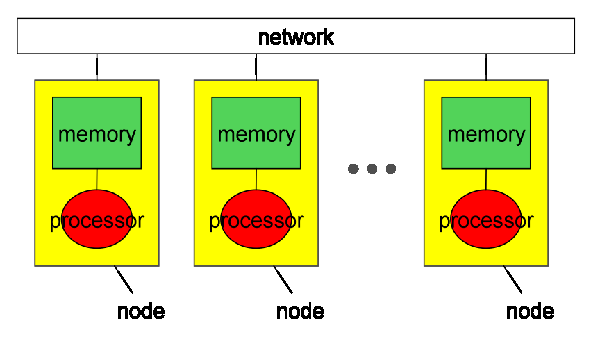
\includegraphics[width=12cm]{figs/Fig1.eps}
  \caption{Hardware Model}\label{fig1}
\end{myfigure}

\section{Execution Model}

The XcalableMP runtime system creates a team of threads on each node
when starting the user program execution. This team of threads is
composed by a single master thread and serveral additional worker
threads.

An XcalableMP program execution is based on the Single Program
Multiple Data (SPMD) model, where the master thread on each node
starts execution from the same main routine and keeps executing the
same code independently (i.e. asynchronously), as if an implicit
tasklet region encloses the whole program, until it encounters an
XcalableMP construct.

The set of nodes on each of which a thread executes a procedure, a
statement, a loop, a block, etc. is referred to as its executing node
set and determined by the innermost task, loop, or array directive
surrounding it dynamically, or at runtime.

The current (executing) node set is the executing node set for the
current context, which is managed by the XcalableMP runtime system on
each node. The current node set at the beginning of the
program execution, or the entire node set, is a node set that contains
all the available nodes, which can be specified in an
implementation-dependent way (e.g. through a command-line option).

When a thread encounters at runtime either a loop, array, or task
construct, and is executed on a node in the node set specified by
the on clause of the directive, it updates the current node set with
the specified one and executes the body of the construct, after which
it resumes the last executing node set and proceeds to execute the
following statements.

Particularly when a thread encounters a loop or an array construct, it
executes the loop body or the array assignment in parallel with
threads on other nodes, so that each iteration of the loop or each
element of the assignment is independently executed on the node where
the specified data element resides.

When a thread encounters a synchronization or a communication
directive, synchronization or communication might occur between it and
threads on other nodes. That is, such global constructs should be
performed collectively on the current nodes. Note that neither
synchronizations nor communications occur without these constructs
specified.

When a thread encounters a tasklet or a taskletloop construct, a new
tasklet is generated on the node. Execution of explicitly generated
tasklets is assigned to one of the threads on the node, subject to the
thread’s availability to execute work. Thus, execution of the new
tasklet could be immediate, or deferred until later according to the
tasklet scheduling constraint and thread availability.

The tasklet scheduling constraint is as follows:

\begin{itemize}
  \item A dependent tasklet shall not be scheduled until its task
		dependences are fulfilled.
\end{itemize}

%%%

% An {\XMP} program execution is based on the Single Program Multiple Data
% (SPMD) model, where each node starts execution from the same main
% routine and keeps executing the same code independently
% (i.e. asynchronously), which is referred to as the {\it \Term{replicated
% execution}}, until it encounters an {\XMP} construct.

% A set of nodes that executes a procedure, a statement, a loop,
% a block, etc. is referred to as its {\it \Term{executing node set}} and
% determined by the innermost {\tt task}, {\tt loop} or {\tt array}
% directive surrounding it dynamically, or at runtime.
% %
% The {\it \Term{current executing node set}} is an executing node set of
% the current context, which is managed by the {\XMP} runtime system on
% each node.

% The current executing node set at the beginning of the program
% execution, or {\it \Term{primary node set}}, is a node set that
% contains all the available nodes, which can be specified in an 
% implementation-dependent way (e.g. through a command-line option).

% When a node encounters at runtime either a {\tt loop}, {\tt array}, or
% {\tt task} construct, and is contained by the node set specified by the
% {\tt on} clause of the directive, it updates the current executing node
% set with the specified one and executes the body of the construct, after
% which it resumes the last executing node set and proceeds to execute the
% following statements.

% Particularly when a node in the current executing node set encounters a
% {\tt loop} or an {\tt array} construct, it executes the loop or the array
% assignment in parallel with other nodes, so that each iteration of the
% loop or element of the assignment is independently executed by the node
% where a specified data element resides.

% When a node encounters a synchronization or a communication directive,
% synchronization or communication occurs between it and other nodes.
% %
% That is, such {\it \Term{global constructs}} are performed collectively
% by the current executing nodes.
% %
% Note that neither synchronizations nor communications occur without these
% constructs specified.

\section{Base Languages}

The XcalableMP language specification is defined on Fortran, C, and C++
as base languages. More specifically, the base language of XcalableMP
Fortran is Fortran 2008, that of XcalableMP C ISO is C99, and that of
XcalableMP C++ is C++11.

\newcommand{\namelistlabel}[1]{\mbox{#1}\hfil}
\newenvironment{namelist}[1]{%
\begin{list}{}
       {\let\makelabel\namelistlabel
        \settowidth{\labelwidth}{#1}
        \setlength{\leftmargin}{1.3\labelwidth}
}
}{%
\end{list}}

\newcommand{\gitem}[1]{\item[{\parbox[b]{3.3cm}{\raggedleft \bf \Term{#1}}}]}


\section{Glossary}\label{sec:glossary}

\subsection{Node Terminology}

\begin{namelist}{entire node setxxxx}

\gitem{node}

  A logical entity managed by the XcalableMP runtime system, which has
  its own local memory and can communicate with each other, and on which
  one or more threads can execute.

\end{namelist}

\subsection{Thread Terminology}

\begin{namelist}{entire node setxxxx}

\gitem{thread}

  An execution entity managed by the XcalableMP runtime system.

\end{namelist}

\subsection{Tasklet Terminology}

\begin{namelist}{entire node setxxxx}

\gitem{tasklet}

  A specific instance of executable code and its data environment,
  generated when a thread encounters a tasklet or taskletloop
  construct.

\end{namelist}

\cleardoublepage

\chapter{Directives}
\index{directive}

\section{Tasklet Constructs}

\subsection{{\tt tasklet} Construct}

\subsubsection*{Synopsis}

% The {\tt \Directive{task}} construct defines a task that is executed by
% a specified node set.

\subsubsection*{Syntax}
\Syntax{tasklet}

\begin{tabular}{ll}
\verb![F]! & \verb|!$xmp| {\tt task on} \{{\it nodes-ref} $\vert$ {\it
 template-ref}\} \\
& {\it structured-block} \\
& \verb|!$xmp| {\tt end task} \\
& \\
\verb![C]! & \verb|#pragma xmp| {\tt task on} \{{\it nodes-ref} $\vert$
     {\it template-ref}\} \\
& {\it structured-block} \\
\end{tabular}

\subsubsection*{Description}

% When a node encounters a {\tt task} construct at runtime, it executes
% the associated block (called a {\it task}) if it is included by the node
% set specified by the {\tt on} clause; otherwise it skips executing the
% block.

% %This line was inserted by Sakagami for svn test. 

% Unless a {\tt task} construct is surrounded by a {\tt \Directive{tasks}}
% construct, {\it nodes-ref} or {\it template-ref} in the {\tt on} clause
% is evaluated by the executing node set at the entry of the task;
% otherwise {\it nodes-ref} and {\it template-ref} of the {\tt task}
% construct are evaluated by the executing node set at the entry of the
% immediately surrounding {\tt tasks} construct.
% %where the evaluation
% %results must be the same in every node in the executing node set.
% %
% The current executing node set is set to that specified by the {\tt on}
% clause at the entry of the {\tt task} construct and rewound to the last
% one at the exit.

% %When {\it nodes-ref} or {\it template-ref} is evaluated, the
% %corresponding new executing node set is created conceptually.

% %The former
% %executing node set that includes the node encountering the {\tt task}
% %construct is referred to as the ``\Term{parent executing node set}'' of
% %the new executing node set.

\subsubsection*{Restrictions}

% \begin{itemize}
% \item The node set specified by {\it nodes-ref} or {\it template-ref}
%       in the {\tt on} clause must be a subset of the parent node set.
% \end{itemize}

% \subsubsection*{Example}
% \Example{task}
% \Example{end task}

% \begin{description}

% \item[Example 1]

% In XcalableMP Fortran, copies of variables {\tt a} and {\tt b} are replicated on
% nodes {\tt nd(1)} through {\tt nd(8)}. 
% A task defined by the {\tt task} construct is executed only on {\tt nd(1)} and
% defines the copies of {\tt a} and {\tt b} on a node {\tt nd(1)}. 
% The copies on nodes {\tt nd(2)} through {\tt nd(8)} are not defined.

% In XcalableMP C, copies of variables {\tt a} and {\tt b} are replicated on
% nodes {\tt nd[0]} through {\tt nd[7]}. 
% A task defined by the {\tt task} construct is executed only on {\tt nd[0]} and
% defines the copies of {\tt a} and {\tt b} on a node {\tt nd[0]}.
% The copies on nodes {\tt nd[1]} through {\tt nd[7]} are not defined.

% \hspace{\hsize}

% \begin{minipage}{0.44\hsize}
% \begin{center}
% \begin{XFexample}
% !$xmp nodes nd(8)
% !$xmp template t(100)
% !$xmp distribute t(block) onto nd

%       real a, b;

% !$xmp task on nd(1)
%       read(*,*) a
%       b = a*1.e-6
% !$xmp end task
% \end{XFexample}
% \end{center}
% \end{minipage}
% %
% \begin{minipage}{0.51\hsize}
% \begin{center}
% \begin{XCexampleR}
% #pragma xmp nodes nd[8]
% #pragma xmp template t[100]
% #pragma xmp distribute t[block] onto nd

%     float a, b;

% #pragma xmp task on nd[0]
%     {
%         scanf ("%f", &a);
%         b = a*1.e-6;
%     }
% \end{XCexampleR}
% \end{center}
% \end{minipage}

% \vspace{1cm}

% \item[Example 2]

% According to the {\tt on} clause with a template reference,
% an assignment statement in the {\tt task} construct is
% executed by the owner of the array element {\tt a(:,j)} or {\tt a[j][:]}.

% \hspace{\hsize}

% \begin{minipage}{0.44\hsize}
% \begin{center}
% \begin{XFexample}
% !$xmp nodes nd(8)
% !$xmp template t(100)
% !$xmp distribute t(block) onto nd

%       integer i,j
%       real a(200,100)
% !$xmp align a(*,j) with t(j)

%       i = ...
%       j = ...

% !$xmp task on t(j)
%       a(i,j) = 1.0
% !$xmp end task
% \end{XFexample}
% \end{center}
% \end{minipage}
% %
% \begin{minipage}{0.51\hsize}
% \begin{center}
% \begin{XCexampleR}
% #pragma xmp nodes nd[8]
% #pragma xmp template t[100]
% #pragma xmp distribute t(block) onto nd

%     int i,j;
%     float a[100][200];
% #pragma align a[j][*] with t[j]

%     i = ...;
%     j = ...;

% #pragma xmp task on t[j]
%     a[j][i] = 1.0;
% }
% \end{XCexampleR}
% \end{center}
% \end{minipage}

% \end{description}


\subsection{{\tt taskletwait} Construct}

\subsubsection*{Synopsis}

% The {\tt \Directive{tasks}} construct is used to instruct the executing
% nodes to execute the multiple tasks it surrounds in arbitrary order.

\subsubsection*{Syntax}
\Syntax{taskletwait}

\begin{tabular}{ll}
\verb![F]! & \verb|!$xmp| {\tt taskletwait} \\
& \\
\verb![C]! & \verb|#pragma xmp| {\tt taskletwait} \\
\end{tabular}

\subsubsection*{Description}

% {\tt \Directive{task}} constructs surrounded by a {\tt tasks} construct
% are executed in arbitrary order without implicit synchronization at the
% entry of each task.
% %
% As a result, if there is no overlap between the executing node sets of
% the adjacent tasks, they can be executed in parallel.

% {\it nodes-ref} or {\it template-ref} of each task immediately
% surrounded by a {\tt tasks} construct is evaluated by the executing node
% set at the entry of the {\tt tasks} construct.

% No implicit synchronization is performed at the entry and exit of the
% {\tt tasks} construct.
% %
% %implicit synchronization is performed at the exit of the {\tt tasks}
% %construct, which guarantees that all communications issued inside child
% %tasks are completed, unless a {\tt nowait} clause is specified.

% %When a {\tt nowait} clause is specified, implicit
% %synchronization is not performed at the end of the {\tt tasks}
% %construct. Without a {\tt nowait} clause, implicit synchronization is
% %performed in order to guarantee that all communications issued inside
% %child tasks are completed.

% \subsubsection*{Example}
% \Example{tasks}
% \Example{task}
% \Example{end tasks}
% \Example{end task}

% \begin{description}
%  \item[Example 1]

% 	    Three instances of subroutine {\tt task1} are concurrently
% 	    executed by node sets {\tt p(1:500)}, {\tt p(501:800)} and
% 	    {\tt p(801:1000)}, respectively.

% \hspace{\hsize}

% \begin{minipage}{0.45\hsize}
% \begin{center}
% \begin{XFexample}
%       subroutine caller
% !$xmp nodes p(1000)
% !$xmp template tp(100)
% !$xmp distribute t(block) onto p
%       real a(100,100)
% !$xmp align a(*,k) with t(k)
%       ...
% !$xmp tasks
% !$xmp  task on p(1:500)
%         call task1(a)
% !$xmp  end task
% !$xmp  task on p(501:800)
%         call task1(a)
% !$xmp  end task
% !$xmp  task on p(801:1000)
%         call task1(a)
% !$xmp  end task
% !$xmp end tasks
%       ...
%       end subroutine
% \end{XFexample}
% \end{center}
% \end{minipage}
% %
% \begin{minipage}{0.45\hsize}
% \begin{center}
% \begin{XFexampleR}
%       subroutine task1(a)
%       ...
% !$xmp nodes q(*)=*

% !$xmp nodes p(1000)
% !$xmp distribute t(block) onto p
%       real a(100,100)
% !$xmp align a(*,k) with t(k)
%       ...
%       end subroutine
% \end{XFexampleR}
% \end{center}
% \end{minipage}

% \vspace{1cm}

%  \item[Example 2]

% 	    The first node {\tt p(1)} executes the first and the second
% 	    tasks, the final {\tt node p(8)} the second and the third
% 	    tasks, and the other nodes {\tt p(2)} through {\tt p(7)}
% 	    only the second task.

% \hspace{\hsize}

% \begin{XFexample}
% !$xmp nodes p(8)
% !$xmp template t(100)
% !$xmp distribute t(block) onto p
%       real a(100)
% !$xmp align a(i) with t(i)
%       ...
% !$xmp tasks

% !$xmp task on t(1)
%       a(1) = 0.0
% !$xmp end task

% !$xmp task on t(2:99)
% !$xmp loop on t(i)
%       do i=2,99
%         a(i) = foo(i)
%       enddo
% !$xmp end task

% !$xmp task on t(100)
%       a(100) = 0.0
% !$xmp end task

% !$xmp end tasks
% \end{XFexample}

% \end{description}


\subsection{{\tt taskletbarrier} Construct}

\subsubsection*{Synopsis}

\subsubsection*{Syntax}
\Syntax{taskletwait}

\begin{tabular}{ll}
\verb![F]! & \verb|!$xmp| {\tt taskletbarrier} \\
& \\
\verb![C]! & \verb|#pragma xmp| {\tt taskletbarrier} \\
\end{tabular}

\subsubsection*{Description}


\cleardoublepage

% \begin{thebibliography}{99}
% \addcontentsline{toc}{chapter}{\bibname}
%  \bibitem{omp} OpenMP Architecture Review Board,
% 	 ``OpenMP Application Program Interface Version 3.1'',
% 	 \url{http://www.openmp.org/mp-documents/OpenMP3.1.pdf}
% 	 (2011).
%  \bibitem{hpf} High Performance Fortran Forum,
% 	 ``High Performance Fortran Language Specification Version 2.0'',
% 	 \url{http://hpff.rice.edu/versions/hpf2/hpf-v20.pdf}
% 	 (1997).
%  \bibitem{mpi} Message Passing Interface Forum,
% 	``MPI: A Message-Passing Interface Standard Version 2.2'',
% 	\url{http://www.mpi-forum.org/docs/mpi-2.2/mpi22-report.pdf}
% 	(2009).
%  \bibitem{hpfja} Japan Association of High Performance Fortran,
% 	 ``HPF/JA Language Specification'',
% 	 \url{http://www.hpfpc.org/jahpf/spec/hpfja-v10-eng.pdf}
% 	 (1999).
%  \bibitem{XPF} Yuanyuan Zhang, Hidetoshi Iwashita, Kuninori Ishii,
% 	 Masanori Kaneko, Tomotake Nakamura, and Kohichiro Hotta,
% 	 ``Hybrid Parallel Programming on SMP Clusters Using XPFortran
% 	 and OpenMP'',
% 	 Proceedings of the International Workshop on OpenMP (IWOMP
% 	 2010), 
% 	 Vol.~6132 of Lecture Notes in Computer Science,
% 	 pp.~133--148,
% 	 Springer
% 	 (2010).
%  \bibitem{VPPFORTRAN} Hidetoshi Iwashita, Naoki Sueyasu, Sachio Kamiya,
% 	 and Matthijs van Waveren,
% 	 ``VPP Fortran and the design of HPF/JA extensions'',
% 	 Concurrency and Computation | Practice \& Experience,
% 	 Vol.~14, No.~8--9, pp.~575--588,
% 	 Wiley
% 	 (2002).
%  \bibitem{OpenMPD} Jinpil Lee, Mitsuhisa Sato, and Taisuke Boku,
% 	 ``OpenMPD: A Directive-Based Data Parallel Language Extension
% 	 for Distributed Memory Systems'',
% 	 Proceedings of the 2008 International Conference on Parallel
% 	 Processing, pp.~121-128
% 	 (2008).
% \end{thebibliography}

\printindex

\end{document}
